% -----------------------------------------------------------------------------
% 1) Paint a story line of developments beginning from SIR
% 2) Give adequate breakdown of types of models:
%.   -  Percolation-based lattice models 
%    -  Non-local dispersal models culminating in the meta-population model
%    -  The continuum-based PDE models ? Spatial SIR models
%.   -  Network models ? 
% 3) Give a breakdown of control methods with these types of models
%.   - Clear examples of how mathematical and computational models inform policy
% -----------------------------------------------------------------------------


\chapter{Modelling infectious tree diseases}

The mathematical and computational modelling of infectious tree diseases began to emerge after Plank had others put forward seminal works on the modelling of crops. Tree disease is import to consider for tree-health in both commercially cultured of stands and naturally occurring forestry and ecosystems. The modelling tree-based disease has many features in common with modelling crop diseases. However, differences in the spatial distribution of hosts and growth cycles remain large.\\

The aim of tree disease modelling is to help design effective control policies. From well designed control policies, the spread of disease through commercial and rural environments can be managed and tree-health maintained. This chapter begins with a chronological overview of tree disease models and the different approaches that have been used in the past.\\

Having reviewed typical models in literature, the theme of control will be reviewed. That is, how the optimal control of a pathogen can be investigated from the construction of models.\\



\section{Modelling approaches to tree-based disease}

The underpinning approaches to tree-based disease were first investigated in the context of crops. At the time computers became commercially viable, research questions could be asked in model simulations \cite{dixon1979spread}. An early simulation-based approach to modelling the spread of tree disease came by \cite{strand1976simulation}. The authors looked considered Western Dwarf Mistletoe \textit{Arceuthobium campylopodum}, an environmentally and economically important plant parasite effecting forest and cultivated stands of ponderosa pine \textit{Pinus pondersa}. A mathematical description was formulated to model the spread, and subsequent increase, of Western Dwarf Mistletoe increase in pine stands. The holistic model given by \cite{strand1976simulation} incorporated a number of \textit{`sub-models'}: crown structure, mistletoe seed production, seed dispersal, reinfection and contagion. The authors modelled the crown structure of pine (i.e. the domed shape of pine), from regression analysis on a sample of pine in the American north-west.\\

 Western Dwarf Mistletoe has an interesting method of `explosive-dispersal', whereby, a ripe fruit builds hydrostatic pressure until seeds are released abruptly to either neighboring branches or individual trees. As such, the authors only took into account explosive dispersal with the assumption that wind-borne and animal-based dispersal negligible. The model ascertained the probability of infection between one mistletoe plant and one branch, located on either the same or different tree. The probability of infection was studied as a function of stand-thinning, to three differently spaced arrangements, alongside the height of infected branches.\\
 
 As we shall see, the type questions asked in this early articles are not seen typical of recent literature. In particular, one does not need to take into account such a fine level of detail when modelling large spatial distances. Mechanistic questions about how the height of infected branches impacts the probability of successful transmission of the parasite.\\
 
 The simulator sub-model approach was also used to by \cite{mcdonald1981computer} to model stem-rust \textit{Cronartium ribicola} in white pines in North America. The authors conducted a detailed model incorporating the full-life cycle of \textit{Cronartium ribicola} and the interplay between two species, pine and ribes.\\
 
\begin{itemize}
    \item  \textcolor{red}{review dutch elm disease as a case study of the different types of models used \cite{doi:10.1098/rstb.1996.0059}}
    \item Explain how planks model falls down with re-infected hosts as a limitation.
\end{itemize}
 




\section{Plant pathology and landscape ecology}
\label{chapter2:plant-ecologoy} 
\textbf{This couples tree disease section to percolation and provides a good intro linking the above paragraph:}
\begin{itemize}
    \item A proper investigation of diseases spread through a tree population cannot be studied in isolation from the landscape. Disease spreads based on the spatial pattern of hosts, heterogeneity of resistance and `reservoir'? Landscape features play an important role in shaping the evolution of the spread. Forest pathology demands a landscape or spatial perspective. Broad scale epidemic (opposed to local outbreaks) require a landscape perspective, see \cite{pub.1012384986} for a review. \textbf{see \cite{pub.1073292723} for an early consideration of spatial considerations... ? double check}
    \item \cite{doi:10.1098/rstb.1998.0226} gave a three population (host, parasite and hyperparasite), which considered transmission via a reaction-diffusion process.
    \item including spatial components within an epidemiological frame-work demanded an interdisciplinary approach between forest pathologists and landscape ecologists, this combined knowledge of plant-based diseases with the methods and tools needed to present a working model in space.
    \item remote sensing tools were used \cite{kelly2002monitoring} to track the study of sudden oak death in California
    \item The need for spatial considerations within disease management was widely accepted at this point,
    \item \cite{kelly2002landscape} demonstrated clustering at the landscape level, spatial structure is important
    \item ... 
    \item various frameworks were put forward, \cite[see][for a detailed analysis]{Gilligan-disease-management}
    \item Percolation theory was used by bailey et al 2000, \textbf{find citations...}
    \item the link between percolation and managing crops were obvious, 
    \item dispersal has been modelled as a random-walk process \cite{PhysRevE.67.031913}
    \item dispersal modelled in relation to heterogeneity?? \cite{CARACO2001185}
    \item anthropogenic factors were noted \cite{doi:10.1890/0012-9658(2002)083[3167:SOAIPO]2.0.CO;2}, along with abiotic factors \cite{doi:10.1046/j.1439-0434.2003.00730.x} such as sunlight intensity ? double check
    \item \cite{doi:10.1046/j.1442-9993.2002.01202.x} the spatial scale is important when modelling the process \cite{spatial-scale}
    \item \textbf{introducing space into the problem lead to percolation...}
\end{itemize}

\textcolor{red}{talk about data:}

Data regarding different tree species distributions will predominantly come in two forms, abundance and presence/absence data. Using abundance data is usually represented in $km^2$ tree cover per hectare (or percentage cover), whereas presence only data only gives binary information if a tree species is present or not.

Abundance data is preferred as more information is captured about the tree species, however, good quality abundance data is in short supply. An interesting model put forward by Louise et at \cite{2STAGE} uses a two stage distribution model. First, presence only data is combined with a series of environmental covariates using a species distribution model in order to produce a map of predicted occurrence data. Random forest regression is then applied to a training sample of real life abundance data producing a high resolution map predicting abundance over the UK at a resolution of $1km^2$. The final result was compared with the remaining abundance data and found to perform much better than existing models. Moving to realistic tree distributions is preferable as the parameter space is reduced by the removal of $\rho$.

\subsection{Spatial scale in tree-based disease}
\cite{https://doi.org/10.1111/jbi.13642}

\subsection{Early warning signals}
\label{section:ews}
\subsection{Percolation\textemdash from forest fires to epidemics}
\label{section:lit-rev-perc}
\begin{figure}
    \centering
    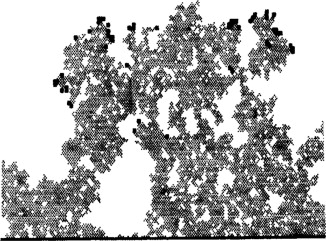
\includegraphics{chapter2/figures/perc1.jpg}
    \caption{A space-time representation of an epidemic spreading at the critical threshold. The spatial (horizontal) and time (vertical) axis show self-similar propagation of diseased individuals in grey, produced by \cite{GRASSBERGER1986273}}
    \label{fig:1d_perc_basis}
\end{figure}

The original formulation of percolation theory was first used to describe properties of a fluid and the bonds which form between molecules \cite{perco_origin} (the reader may jump to \ref{fig:ch3-perc-invariance} for an account of percolation). The problem was posed on a graph\textemdash illustrated in terms of vertices and edges. However re-interpretations were subsequently put forward by physicists studying material sciences, naturally on a lattice. \cite{Essam_1980}. The attractive feature of this new paradigm was that percolation demonstrated a phase-transition. Thus, percolation could be treated with scaling theory used in the study of critical-phenomena. Accordingly, early work rigorously ensued to map out the behaviour of percolation around criticality in terms of critical exponents \cite{STAUFFER19791}. 

Different flavours of percolation models, such as, site or bond percolation were described to model different processes. Percolation proved a convenient theory and various phenomena including, gelation, magnetism and telecommunications were described \cite{trove.nla.gov.au/work/26493727}. Interestingly, forest fires were also applicable to a description within percolation theory \cite{MacKay_1984}. This was a short conceptual jump from time-dependant percolation used to study the growth of crystals \cite{Family_1985}. 

A fire spreading through a population of trees is not to dissimilar to a disease spreading through a population. This lead to a general epidemic-formalisation within percolation-based framework when \cite{pub.1059067807} argued that epidemics were in the same universality class as percolation. It is alluring to remark how modelling the same processes with different microscopic interactions (e.g. different lattice geometries) lead to the macroscopic behaviour should they have the same universality class\textemdash see chapter \ref{fig:ch3-perc-invariance} for more information.

Beginning with a simple $SIR$ framework put forward by \cite{kermack-model}, the field of epidemiology was already well established around the time percolation theory was conceived \cite{baily1975mathematical}. In particular, initial assumptions about population mixing could be relaxed with more elaborate spatial-contact models, naturally, percolation theory could serve as a useful tool when developing spatially-structured epidemic models.

A fractal-like pattern of epidemics was observed by \cite{GRASSBERGER1986273}, shown in Figure \ref{fig:1d_perc_basis}. Parsimoniously describing Figure \ref{fig:1d_perc_basis}, lighter grey sites represent removed individuals, black sites indicate actively infected sites and white sites indicate unaffected sites. All lattice sites in the bottom row were initially infected and the infection can be seen to propagate from the bottom up. The lattice was initialised at the critical-density $p\sim p_c$ culminating in a fractal-like pattern. \cite{GRASSBERGER1986273} did not attribute the hosts of this model to be trees, but instead a general host-population with very low mobility. Local interactions between hosts and infected were elucidated as vast simplifications and long-range interactions (following a power-law) were discussed\textemdash we shall see how these ideas form a important component of modelling tree disease.

The behaviour of percolation-based epidemic models continued (e.g. \cite{pub.1060474189, pub.1059069981}) to be investigated with various methods such as renormalisation-groups and Monte-Carlo, the critical exponents were found along with phase transition graphs characterising epidemic (super-critical) or extinction (sub-critical) regimes. The properties of both epidemics and forest fire percolation models were studied together in \cite{pub.1052857560}, highlighting their similarity.

The first ecological application came in \cite{pub.1031591030} where forest fire (and epidemic) percolation models were adapted in order to study landscape disturbances. Broadly speaking, landscape disturbances constitute a broad array of physical process which lead to a rapid ecological change, this could include invasion of pests, climate-change and fire.

\textemdash\cite{GRASSBERGER1983157} <- reference for early considerations towards percolation as a model for tree diseases and percolation
\textemdash\cite{SANDER2002293}, read and get more info + research links

\subsection{Metapopulation}

\begin{itemize}
    \item this variation in epidemic outcome from variants of environmental factors was likened to the metapopulation used in ecology and population dynamics in order to describe environment `patchiness'
    \item variability in the host landscape was considered and recognised as important, the patchiness of a landscape lends itself well to a metapopulation model
    \cite{doi:10.1098/rstb.1986.0072}

\end{itemize}
\subsection{Continuum modelling and spatial SIR}
\begin{itemize}
    \item \textcolor{red}{Murray}: travelling waves do not change shape
\end{itemize}

\subsection{Network modelling for human-mediated transport}
\blindtext[1]

\section{Controlling Plant-Based Epidemics\textemdash a review}

- Re-draft and check the above, remove unnecessary paragraphs i.e. crop out some computational modelling... Then: 1) Literature review of plant disease models 2) Review of control methods.

\section{Chapter summary}